Every chapter so far assumes access to a scalar reward signal. Dynamic programming (Chapter 3) requires the full reward function $r(s,a)$. Model-free RL (Chapter 2) relaxes the model requirement but still observes a numerical reward $r_t$ after each transition. Q-learning, temporal difference methods, policy gradient, all update toward a scalar signal. The Bellman optimality equation $V^*(s) = \max_a \{r(s,a) + \gamma \sum_{s'} P(s'|s,a) V^*(s')\}$ presupposes that $r(s,a)$ is either known or observable. When it is neither, the entire DP/RL machinery cannot be applied directly.

In many domains, scalar rewards are unavailable but ordinal preferences over trajectories are easy to elicit. Text generation is the canonical example: a human evaluator cannot assign a meaningful numerical score to a paragraph of text, but can reliably say ``response A is better than response B'' when shown two candidate completions. Similarly, in robotics, a human can compare two demonstrated behaviors without specifying a cost function. The raw data in RLHF is a set of trajectory pairs (or trajectory segment pairs) with binary preference labels indicating which trajectory the evaluator preferred. RLHF uses these ordinal comparisons to learn a proxy reward function $r_\theta$, which then serves as the scalar signal for standard RL optimization. This is not an inverse problem in the IRL sense; the goal is not to rationalize observed behavior or recover the agent's own reward, but rather a two-stage forward problem: first learn a reward from human judgments, then solve the resulting MDP using the RL tools from earlier chapters.

When no one can write down the reward function, human preferences provide an alternative training signal. Reinforcement Learning from Human Feedback (RLHF) learns a reward function by eliciting pairwise preference comparisons from a human evaluator over machine-generated outputs, rather than inverting an observed policy as in structural estimation or IRL. \citet{christiano:2017} demonstrated that this approach could train agents without an explicit reward function. RLHF has since become the predominant method for aligning large language models.

\subsection{Learning Rewards from Preferences}

The canonical RLHF framework is built on a formal model of human preference. The observed data consists of tuples $(s, y_w, y_l)$, where $s$ is a context, and $y_w$ and $y_l$ are two outputs, with $y_w$ being the ``winner'' preferred by a human. Assuming preferences follow a latent utility model, the Bradley-Terry model \citep{bradley1952rank} gives the probability that $y_w$ is preferred: $P(y_w \succ y_l | s) = \sigma(r_\theta(s, y_w) - r_\theta(s, y_l))$, where $r_\theta: \mathcal{S} \times \mathcal{Y} \to \mathbb{R}$ is a learned reward model parameterized by $\theta$, trained to approximate human preferences (not the ground-truth reward, which is unobserved), and $\sigma(\cdot)$ is the logistic function. This formulation is a direct application of discrete choice theory and is equivalent to a binary logit model, a special case of the multinomial logit framework \citep{mcfadden:1973} that underpins DDC estimation. The reward model parameters $\theta$ are estimated by minimizing the negative log-likelihood of the observed human choices:
\begin{equation}
    \mathcal{L}(\theta) = -\mathbb{E}_{(s, y_w, y_l) \sim \mathcal{D}} \left[ \log \sigma \left( r_\theta(s, y_w) - r_\theta(s, y_l) \right) \right],
\label{eq:rlhf_loss}
\end{equation}
In the LLM setting, the ``outputs'' $y_w$ and $y_l$ are token sequences, i.e., trajectories of the autoregressive policy, so preferences are over trajectories rather than single actions. The preference loss in Equation~(\ref{eq:rlhf_loss}) is MLE of a choice model where the ``alternatives'' are trajectory segments and the ``choice'' is the human-preferred one.

\subsection{The RLHF Pipeline and Direct Optimization}

The learned $r_\theta$ then serves as a proxy objective for policy optimization. Building on the reward-learning and RL fine-tuning framework of \citet{ziegler2019fine} and \citet{stiennon2020learning}, the canonical three-stage pipeline was formalized by \citet{ouyang2022training}. First, a base pretrained model is initialized via supervised fine-tuning (SFT) on a small dataset of high-quality demonstrations, yielding an initial policy $\pi^{SFT}$. This grounds the model in the desired style and format. The second step is the reward model training as described, using preference data generated from this $\pi^{SFT}$.

In the third and final step, the policy is optimized using reinforcement learning. The $\pi^{SFT}$ policy, now denoted $\pi_\phi$, is fine-tuned to maximize the expected reward signal from the frozen reward model $r_\theta$. In practice, this optimization uses PPO (Chapter 2, Section 5), the same clipped policy gradient method that stabilizes updates via a trust region. The standard policy gradient machinery from Chapter 2 applies directly, with one twist: the reward function is itself an estimate, introducing approximation error on top of the usual variance in gradient estimates. A critical component of this optimization is the inclusion of a regularization term that penalizes the Kullback-Leibler (KL) divergence between the learned policy $\pi_\phi$ and the initial reference policy $\pi^{SFT}$. The objective function for this final stage is:
\begin{equation}
    J(\phi) = \mathbb{E}_{s \sim \mathcal{D}, y \sim \pi_\phi(\cdot|s)} [r_\theta(s, y)] - \lambda_{KL} \mathbb{E}_{s \sim \mathcal{D}} [D_{KL}(\pi_\phi(\cdot|s) \,||\, \pi^{SFT}(\cdot|s))],
\label{eq:rlhf_objective}
\end{equation}
where $D_{KL}$ is the Kullback-Leibler divergence and $\lambda_{KL}$ is a hyperparameter controlling the penalty strength.\footnote{$\lambda_{KL}$ denotes the KL penalty weight, reserving $\beta$ for model parameters and $\gamma$ for discount factors. The standard RLHF literature, including \citet{rafailov2023direct}, uses $\beta$ for this parameter.} This KL-divergence term is essential because it prevents the policy $\pi_\phi$ from deviating too far from the distribution of text on which the reward model is reliable, thus mitigating ``reward hacking'' where the policy exploits inaccuracies in $r_\theta$ to achieve a high score with degenerate behavior. The KL regularization serves a function analogous to the stabilization techniques discussed in Chapter 3's treatment of the deadly triad: it constrains the policy to regions where the learned reward model $r_\theta$ is reliable, preventing the RLHF analogue of divergence under function approximation.

The KL-regularized objective in Equation~(\ref{eq:rlhf_objective}) admits a Bayesian interpretation \citep{korbak2022rl}. In this view, the reference policy $\pi^{SFT}$ acts as a prior distribution over plausible responses. The reward model $r_\theta$ provides evidence, specifying which responses are more desirable. The goal of alignment is to find the posterior distribution $\pi^*$ that optimally combines the prior with this evidence. This ideal posterior policy takes the form of Equation~(\ref{eq:rlhf_posterior}):
\begin{equation}
    \pi^*(y|s) \propto \pi^{SFT}(y|s) \exp\left(\frac{r_\theta(s, y)}{\lambda_{KL}}\right).
\label{eq:rlhf_posterior}
\end{equation}
This formulation directly parallels Bayes' rule, where the posterior is proportional to the prior times the likelihood. The reward function, scaled by $\lambda_{KL}$, defines the log-likelihood of the preference evidence. From this perspective, the KL-regularized RL objective $J(\phi)$ is no longer arbitrary. It is mathematically equivalent, up to an additive constant, to the Evidence Lower Bound (ELBO) for this Bayesian inference problem. Consequently, maximizing the RLHF objective via PPO is a form of variational inference, where the aim is to find the policy $\pi_\phi$ that minimizes the KL divergence to the ideal posterior $\pi^*$. This insight reframes RLHF from a reward-maximization task into a probabilistic inference problem, providing a theoretical justification for the KL penalty as a structural component of the inference problem rather than an ad-hoc regularizer.

Despite this closed-form characterization, the three-stage RLHF pipeline is complex to implement, requiring training multiple large models and a computationally expensive reinforcement learning loop that involves sampling from the policy. Building on the analytical relationship between the optimal policy and the reward function, Direct Preference Optimization (DPO) was introduced by \citet{rafailov2023direct} as a simpler, RL-free method. DPO eliminates the RL optimization loop entirely, bypassing the policy gradient and value function machinery of Chapters 2 and 3. Where standard RLHF decomposes the problem into ``learn reward from trajectory preferences'' then ``solve the resulting MDP,'' DPO solves for the policy directly from the same preference data over trajectory pairs, collapsing two stages into one supervised learning objective. DPO bypasses the explicit reward modeling step by reparameterizing the reward function directly in terms of the optimal policy $\pi^*$ and the reference policy $\pi^{SFT}$, as in Equation~(\ref{eq:dpo_reparameterize}):
\begin{equation}
    r(s,y) = \lambda_{KL} \log\left(\frac{\pi^*(y|s)}{\pi^{SFT}(y|s)}\right) + \lambda_{KL} \log Z(s).
\label{eq:dpo_reparameterize}
\end{equation}
When this analytical expression for the reward is substituted into the Bradley-Terry preference loss from Equation~(\ref{eq:rlhf_loss}), the unknown partition function $Z(s)$ cancels out. This yields a loss function that depends only on the policy $\pi_\phi$ being optimized and the fixed reference policy $\pi^{SFT}$. The DPO objective, given in Equation~(\ref{eq:dpo_loss}), is thus a simple binary cross-entropy loss over policy likelihoods:
\begin{equation}
    \mathcal{L}_{DPO}(\phi; \pi^{SFT}) = -\mathbb{E}_{(s, y_w, y_l) \sim \mathcal{D}} \left[ \log \sigma \left( \lambda_{KL} \log \frac{\pi_\phi(y_w|s)}{\pi^{SFT}(y_w|s)} - \lambda_{KL} \log \frac{\pi_\phi(y_l|s)}{\pi^{SFT}(y_l|s)} \right) \right].
\label{eq:dpo_loss}
\end{equation}
This objective can be optimized directly on the policy parameters $\phi$ using standard supervised learning techniques with a static preference dataset. The gradient of this loss intuitively increases the likelihood of preferred responses $y_w$ while decreasing the likelihood of dispreferred responses $y_l$, relative to the reference policy. By recasting the constrained optimization problem as a simple likelihood maximization, DPO offers a more stable and computationally efficient alternative to the multi-stage RLHF pipeline, eliminating the need for an explicitly trained reward model and the complexities of RL-based policy optimization.

\subsection{Recent Developments}

A subsequent innovation leverages DPO to create an iterative self-improvement loop, reducing reliance on static, human-annotated data \citep{yuan2024self}. In this paradigm, dubbed Self-Rewarding Language Models, a single language model acts as both the instruction-following agent and its own reward model. The process begins with a base model fine-tuned to have both instruction-following and evaluation capabilities (``LLM-as-a-Judge''). In each subsequent iteration, the current model generates a new preference dataset for itself by producing multiple responses to a set of prompts and then evaluating its own outputs to assign scores. These scores are used to construct preference pairs $(y_w, y_l)$, which form an AI-generated feedback dataset. The model is then fine-tuned on this new data using the DPO loss. This iterative process creates a feedback loop where enhancements in instruction-following ability lead to better reward modeling, which in turn fuels the next round of policy optimization.

While RLHF and its successors have proven effective at aligning model behavior with human preferences, several open issues remain. The framework does not aim to solve the identification problem in the strict econometric sense; the learned reward model $r_\theta$ (whether explicit or implicit in DPO) is a proxy for preference, not necessarily the uniquely identified ``true'' utility function required for welfare analysis.\footnote{The identification problem in preference learning mirrors that in discrete choice. The reward function is identified only up to an additive constant and requires a location normalization.} Furthermore, the notion of ``human feedback'' is a significant simplification, as the preferences being optimized are those of a small, non-representative group of paid labelers, raising important questions about whose values are being embedded in these systems. Finally, the fine-tuning process can lead to degraded performance on standard academic benchmarks, a phenomenon called the ``alignment tax'' \citep{ouyang2022training}.\footnote{The alignment tax, as described by \citet{ouyang2022training}, refers to performance regressions on public NLP benchmarks (SQuAD, DROP, HellaSwag) that result from RLHF fine-tuning.} Mitigating these challenges while scaling alignment beyond the limits of human data collection remains a key frontier for the field.

\subsection{Simulation Study: Learning from Preferences on a Gridworld}

The gridworld is a $10 \times 10$ stochastic grid with slip probability $p = 0.1$ and discount factor $\gamma = 0.99$, structurally identical to the environments in Chapters 3a and 4. The agent starts at $(0,0)$ and must reach the goal at $(9,9)$, receiving $r = -0.1$ per step, $r = +10$ for reaching the goal, $r = -2$ for entering hazard cells at $(3,3)$ and $(6,7)$, and $r = -5$ for entering a trap at $(5,2)$. The true reward function is linear in four indicator features, $r(s,a,s') = \phi_0 + \phi_1 \mathbbm{1}\{s' = \text{goal}\} + \phi_2 \mathbbm{1}\{s' \in \text{hazards}\} + \phi_3 \mathbbm{1}\{s' \in \text{traps}\}$, with $\phi = (-0.1, 10.1, -1.9, -4.9)$. Dynamic programming gives $V^*(s_0) = 6.55$; the optimal policy avoids all hazards and traps. Figure~\ref{fig:rlhf_env} shows the environment with $V^*(s)$ and $\pi^*$.

\begin{figure}[htbp]
\centering
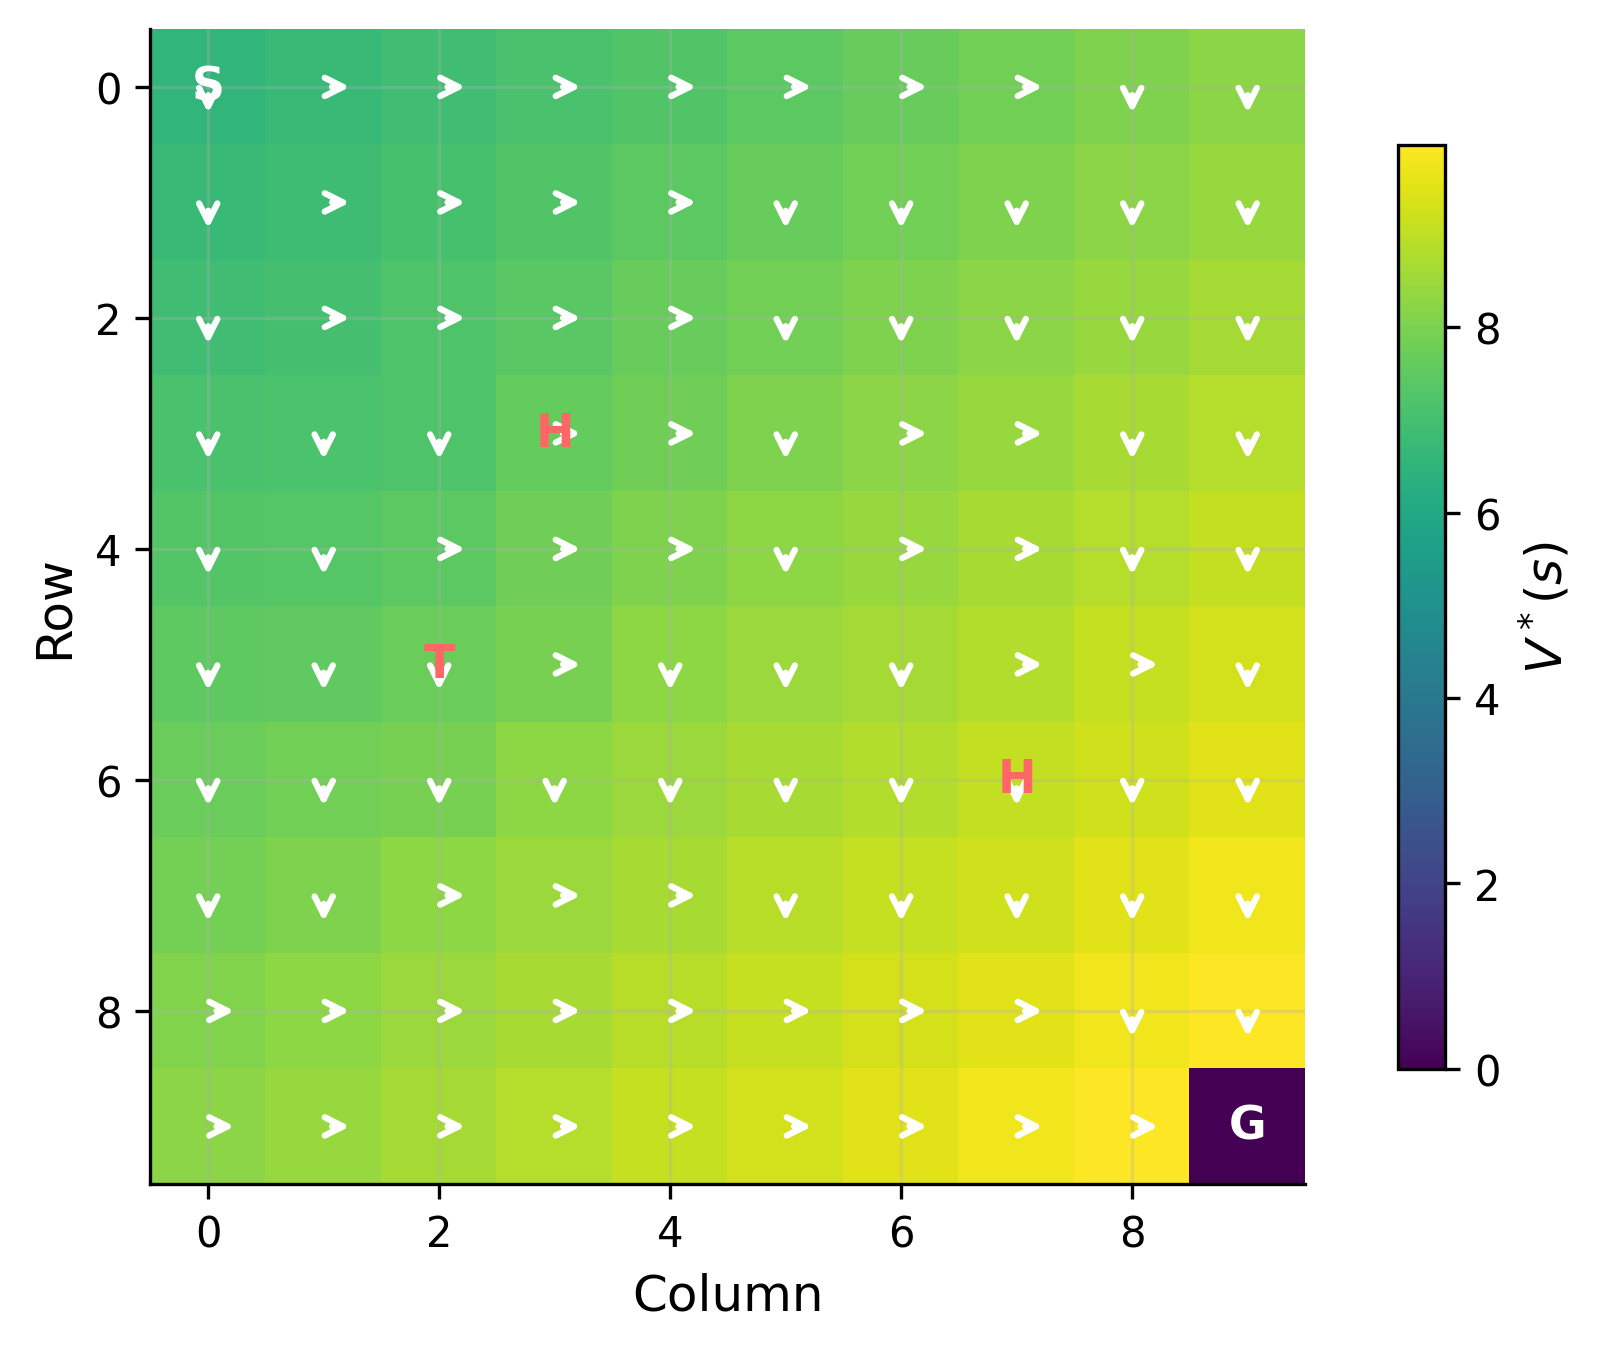
\includegraphics[width=0.7\textwidth]{ch08_rlhf/sims/gridworld_rlhf_env.png}
\caption{The $10 \times 10$ stochastic gridworld. Cell shading shows $V^*(s)$ (viridis scale); arrows indicate the optimal policy $\pi^*$. S marks the start, G the goal, H the hazard cells, and T the trap. The optimal policy routes right and down toward the goal while steering around hazards and traps.}
\label{fig:rlhf_env}
\end{figure}

Preference data is generated by rolling out a uniform random policy (each action equally likely) from random non-goal start states. Each rollout produces a trajectory segment of $L = 25$ steps. For each of $K$ comparisons, two independent segments are generated; the segment with higher cumulative reward under the true (unobserved) reward function is labeled as preferred via the Bradley-Terry model. This produces $K$ binary comparisons. All six methods receive identical preference data per seed; the agent never observes per-transition rewards, only the binary preference label per pair.

Five methods are compared across $K \in \{25, 50, 100, 200, 500, 1000, 2000, 5000\}$, averaged over 30 seeds. The neural network RLHF reward model is a two-layer MLP (8 inputs encoding normalized row and column positions plus one-hot action, 64 hidden units, $\sim$4,800 parameters) trained by Bradley-Terry MLE on the $K$ segment pairs. For each segment, the model computes per-transition rewards $r_\theta(s_t, a_t, s_{t+1})$ and sums them to obtain a segment score; the preferred segment should score higher under the logistic loss from Equation~(\ref{eq:rlhf_loss}). After 200 training epochs (learning rate $10^{-3}$, batch size 64), the $100 \times 4$ reward table is extracted and the resulting MDP solved by value iteration. The correctly specified structural model parameterizes reward as $r = \phi_0 + \phi_1 \mathbbm{1}\{\text{goal}\} + \phi_2 \mathbbm{1}\{\text{hazard}\} + \phi_3 \mathbbm{1}\{\text{trap}\}$ (4 parameters matching the true form); $\phi$ is fit by L-BFGS-B maximization of the same Bradley-Terry log-likelihood, and the resulting MDP solved by value iteration. The misspecified variant uses only $\phi_0$ and $\phi_1$, ignoring hazards and traps. Tabular Q-learning (20,000 episodes, $\varepsilon = 0.1$, $\alpha = 0.1$) and exact DP provide scalar-reward baselines that observe per-transition rewards.

\begin{table}[htbp]
\centering
\caption{Sample complexity of preference-based policy learning on a stochastic $10 \times 10$ gridworld (30 seeds). The neural network reward model reaches 99\% of DP-optimal at $K = 1{,}000$. The correctly specified structural model reaches 100\% at $K = 5{,}000$ but has high variance at intermediate $K$. The misspecified model plateaus near 98\% while routing through hazard cells.}
\label{tab:rlhf_gridworld}
\begin{tabular}{llrr}
\hline
Method & $K$ & Return & \% of DP \\
\hline
DP Oracle & --- & $6.52 \pm 0.02$ & $100.0$ \\
Q-Learning & --- & $6.50 \pm 0.01$ & $99.7$ \\
\hline
NN RLHF & $25$ & $-6.28 \pm 1.29$ & $-96.3$ \\
Correct & $25$ & $4.89 \pm 0.90$ & $75.0$ \\
Misspecified & $25$ & $4.79 \pm 0.90$ & $73.5$ \\
\hline
NN RLHF & $50$ & $-3.37 \pm 1.43$ & $-51.6$ \\
Correct & $50$ & $6.00 \pm 0.54$ & $92.0$ \\
Misspecified & $50$ & $5.89 \pm 0.54$ & $90.2$ \\
\hline
NN RLHF & $100$ & $3.06 \pm 1.19$ & $47.0$ \\
Correct & $100$ & $4.35 \pm 1.02$ & $66.6$ \\
Misspecified & $100$ & $4.81 \pm 0.90$ & $73.8$ \\
\hline
NN RLHF & $200$ & $4.75 \pm 0.90$ & $72.8$ \\
Correct & $200$ & $4.90 \pm 0.90$ & $75.2$ \\
Misspecified & $200$ & $4.82 \pm 0.90$ & $73.8$ \\
\hline
NN RLHF & $500$ & $6.21 \pm 0.27$ & $95.1$ \\
Correct & $500$ & $4.89 \pm 0.90$ & $75.0$ \\
Misspecified & $500$ & $4.78 \pm 0.90$ & $73.3$ \\
\hline
NN RLHF & $1000$ & $6.45 \pm 0.04$ & $98.9$ \\
Correct & $1000$ & $5.46 \pm 0.75$ & $83.6$ \\
Misspecified & $1000$ & $5.89 \pm 0.54$ & $90.3$ \\
\hline
NN RLHF & $2000$ & $6.52 \pm 0.01$ & $99.9$ \\
Correct & $2000$ & $6.01 \pm 0.54$ & $92.1$ \\
Misspecified & $2000$ & $6.44 \pm 0.02$ & $98.7$ \\
\hline
NN RLHF & $5000$ & $6.48 \pm 0.01$ & $99.4$ \\
Correct & $5000$ & $6.55 \pm 0.00$ & $100.4$ \\
Misspecified & $5000$ & $6.42 \pm 0.02$ & $98.4$ \\
\hline
\end{tabular}

\end{table}

Table~\ref{tab:rlhf_gridworld} and Figure~\ref{fig:rlhf_sample} report the main results. The neural network reward model converges fastest, rising from negative returns at $K = 25$ to 95\% of DP-optimal at $K = 500$ and 99\% at $K = 1{,}000$. The correctly specified structural model dominates at very low $K$ (75\% at $K = 25$ versus $-96\%$ for the neural net) but exhibits high variance at intermediate $K$ (standard errors of $\pm 0.9$), because hazard and trap cells constitute only 3 of 99 non-terminal states and random segments rarely visit them, leaving $\phi_2$ and $\phi_3$ poorly identified.\footnote{At $K = 100$, the estimated trap penalty $\hat{\phi}_3 = -18.6$ overshoots the true value of $-4.9$ by a factor of four, causing the policy to take extreme detours.} At $K = 5{,}000$, the structural model achieves 100.4\% of DP return with parameter estimates converging toward their true values. The misspecified model converges to 98.4\%, a seemingly small gap, but its policy consistently routes through hazard cells (2.1 visits on average), confirming qualitative misspecification.\footnote{The modest return gap arises because hazard penalties ($-2$ per visit, $\sim$2 visits per episode) are small relative to total return ($\sim$6.5). Larger penalties or more hazards would widen it.} Q-learning converges to 99.7\% of DP using 458,000 scalar reward observations, three orders of magnitude more signal than the neural net requires at $K = 1{,}000$. The flexible neural net outperforms the correctly specified structural model at intermediate sample sizes ($K = 500$ through $K = 2{,}000$) because its 8-dimensional input representation extracts reward information from every transition, not just the rare visits to 3 special cells. Even mild misspecification (omitting 2 of 4 reward features) produces qualitatively wrong policies despite quantitatively similar returns.

\begin{table}[htbp]
\centering
\caption{Diagnostics at $K = 5{,}000$ (single seed). Policy agreement measures the fraction of non-goal states where each method's greedy policy matches $\pi^*$. Reward MAE is the mean absolute error of the estimated expected reward table against the true table. $V^\pi$ correlation is the Pearson correlation between the true value of the learned policy (evaluated under the true reward) and $V^*$. Hazard visits counts states where the deterministic policy routes into hazard or trap cells.}
\label{tab:rlhf_diagnostics}
\begin{tabular}{lrrrr}
\hline
Method & Policy agreement (\%) & Reward MAE & $V^\pi$ corr.\ with $V^*$ & Hazard visits \\
\hline
NN RLHF & $77.8$ & $0.766$ & $0.836$ & $1$ \\
Correct & $100.0$ & $0.081$ & $1.000$ & $0$ \\
Misspecified & $77.8$ & $0.190$ & $0.809$ & $2$ \\
\hline
\end{tabular}

\end{table}

Table~\ref{tab:rlhf_diagnostics} provides a different view of the $K = 5{,}000$ results, showing what each method actually learned rather than just policy returns. The correctly specified structural model achieves 100\% policy agreement with $\pi^*$ and value function correlation 1.000, recovering the true reward to within MAE 0.081. The neural network model, despite achieving 99\% of DP return in the main experiment, agrees with $\pi^*$ on only 78\% of states; the disagreements occur at states far from the typical trajectory where the precise action choice has little impact on expected return. The misspecified model matches the neural net in policy agreement (78\%) but for a different reason; it routes through hazard cells that the optimal policy avoids, producing a qualitatively distinct trajectory distribution with value function correlation 0.809.
\begin{table}[htbp]
\centering
\caption{Online versus offline data collection for the neural network RLHF model at $K = 1{,}000$ (20 seeds). Online collection is unstable; catastrophic failures on approximately half of seeds produce a negative mean return.}
\label{tab:rlhf_online_offline}
\begin{tabular}{lrr}
\hline
Collection & Return & $p$-value \\
\hline
Online (4 rounds) & $-2.59 \pm 1.81$ & \\
Offline & $5.82 \pm 0.66$ & $0.9999$ \\
\hline
\end{tabular}

\end{table}

Table~\ref{tab:rlhf_online_offline} reports the online versus offline ablation for the neural network model at $K = 1{,}000$. The online procedure divides $K$ into four rounds of 250 comparisons each, collecting subsequent rounds from the current learned policy rather than the random policy. Offline collection ($5.82 \pm 0.66$) substantially outperforms online ($-2.59 \pm 1.81$, $p > 0.999$). A poor first-round reward model, trained on only 250 comparisons, produces a degenerate policy whose concentrated state visitation degrades subsequent rounds through a compounding feedback loop. In this gridworld, the random policy already provides near-uniform state coverage that targeted collection can only narrow. The finding contrasts with \citet{christiano:2017}, where online collection helped in high-dimensional Atari and MuJoCo environments because random exploration fails to cover the relevant state space; in small, well-covered environments, the instability risk of online collection outweighs its potential benefit.

\begin{figure}[htbp]
\centering
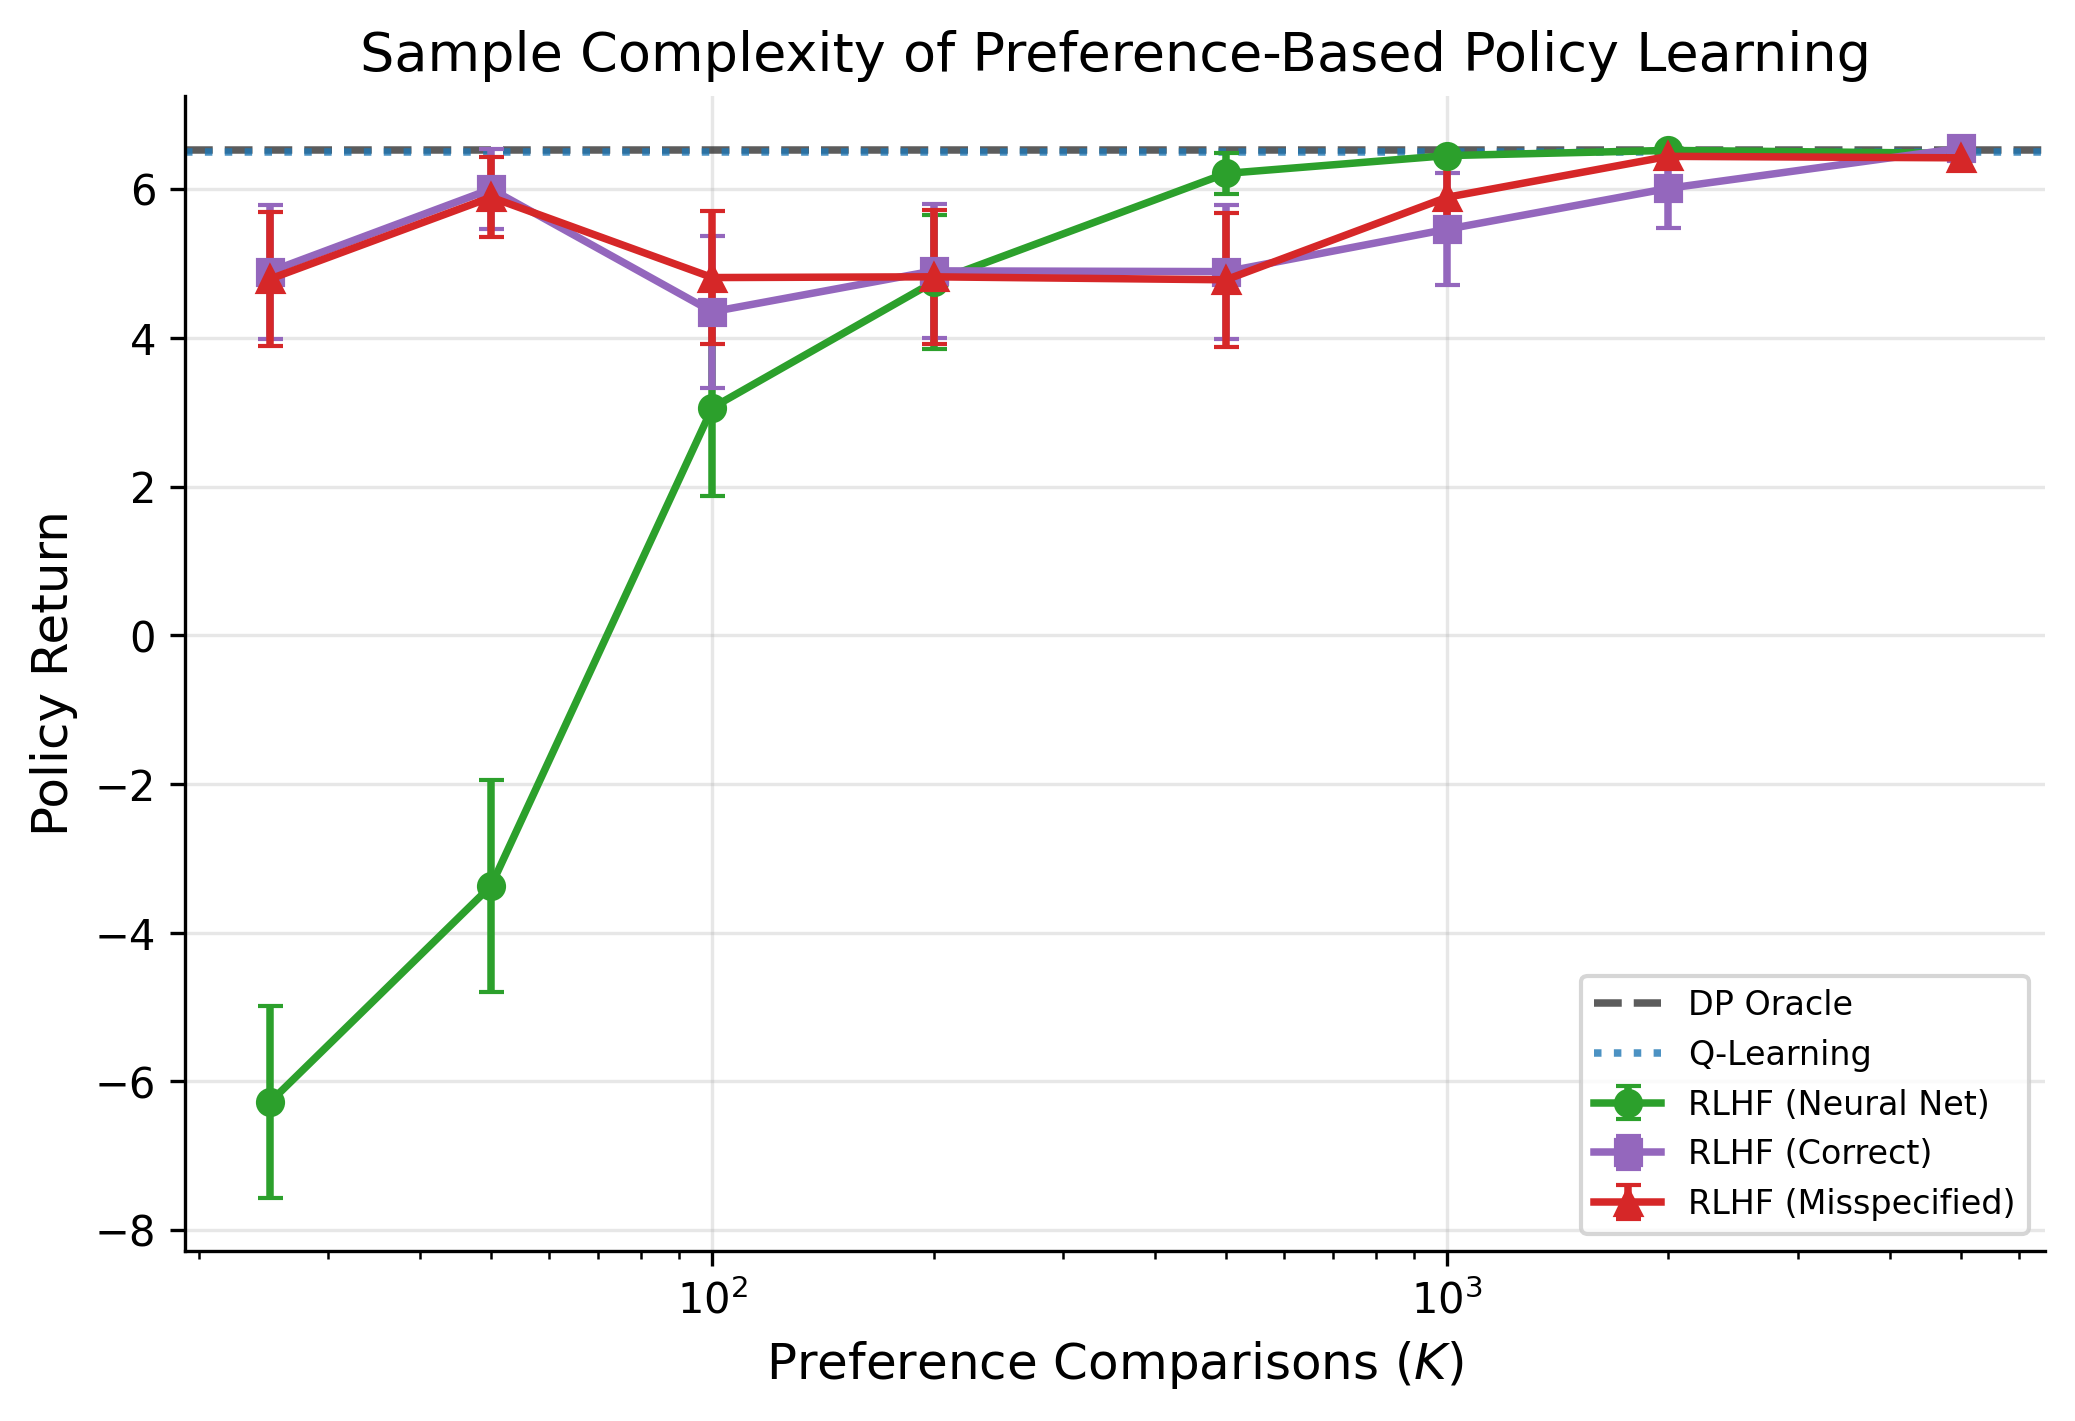
\includegraphics[width=0.7\textwidth]{ch08_rlhf/sims/gridworld_sample_complexity.png}
\caption{Policy return versus number of preference comparisons. The neural network RLHF model ($\sim$4,800 parameters) converges fastest to near-optimal return. The structural model (4 parameters) has high variance at intermediate $K$ but achieves exact recovery at $K = 5{,}000$.}
\label{fig:rlhf_sample}
\end{figure}

